\section{Introduction}
\label{sec:intro}
% Editors: Brendan McMahan (mcmahan)
% Other contributors: Dave

Federated learning (FL) is a machine learning setting where many clients (e.g. mobile devices or whole organizations) collaboratively train a model under the orchestration of a central server (e.g. service provider), while keeping the training data decentralized. It embodies the principles of focused collection and data minimization, and can mitigate many of the systemic privacy risks and costs resulting from traditional, centralized machine learning. This area has received significant interest recently, both from research and applied perspectives. This paper describes the defining characteristics and challenges of the federated learning setting, highlights important practical constraints and considerations, and then enumerates a range of valuable research directions. The goals of this work are to highlight research problems that are of significant theoretical and practical interest, and to encourage research on problems that could have significant real-world impact.

联邦学习(FL)是一种机器学习设置, 其中许多客户端(例如移动设备或整个组织)在中央服务器(例如服务提供商)的协调下协作培训模型, 同时保持培训数据的分散. 它体现了集中收集和数据最小化的原则, 可以减轻传统集中式机器学习带来的许多系统性隐私风险和成本. 从研究和应用的角度来看, 这一领域最近受到了极大的关注. 本文描述了联邦学习环境的定义特征和挑战, 强调了重要的实践约束和注意事项, 然后列举了一系列有价值的研究方向. 这项工作的目标是突出具有重大理论和实践意义的研究问题, 并鼓励对可能产生重大现实影响的问题进行研究. 

The term \emph{federated learning} was introduced in 2016 by \citet{mcmahan17fedavg}: ``We term our approach Federated Learning, since the learning task is solved by a loose federation of participating devices (which we refer to as clients) which are coordinated by a central server.''  An unbalanced and non-IID (identically and independently distributed) data partitioning across a massive number of unreliable devices with limited communication bandwidth was introduced as the defining set of challenges.
% Work this footnote in if we can find a suitable citation (mcmahan - i couldn't find a good one).
% \footnote{This motivated the choice of the term ``federated'' which can be defined for example as ``a group of states with a central government but independence in internal affairs.''\todo{Citation}}

术语\emph{federated learning}于2016年由\citet{mcmahan17fedavg}引入, ``我们将我们的方法称为联邦学习, 因为学习任务由参与设备(我们称之为客户端)的松散联盟解决, 这些设备由中央服务器协调." 一个不平衡的非IID在通信带宽有限的大量不可靠设备之间进行(相同且独立分布)数据分区是一组确定的挑战. 

%如果我们能找到一个合适的引文, 就把这个脚注写进去(mcmahan——我找不到一个好的引文). 
%\footnote{这促使人们选择了“联邦”一词, 例如可以将其定义为“一个拥有中央政府但在内部事务中独立的国家集团”. \todo{引文}

Significant related work predates the introduction of the term federated learning. A longstanding goal pursued by many research communities (including cryptography, databases, and machine learning) is to analyze and learn from data distributed among many owners without exposing that data. Cryptographic methods for computing on encrypted data were developed starting in the early 1980s \citep{Rivest1978,yao1982protocols}, and \citet{agrawal2000} and \citet{vaidya2008ppsvm} are early examples of work that sought to learn from local data using a centralized server while preserving privacy.
%
重要的相关工作早于联邦学习这一术语的引入. 这是许多研究团体(包括密码学、数据库和机器学习)追求的长期目标是从分布在许多所有者之间的数据中进行分析和学习, 而不公开这些数据. 加密数据的加密计算方法是从1980年代初开始开发的\citep{Rivest1978,yao1982protocols}, 以及\citet{agrawal2000}和\citet{vaidya2008ppsvm}是早期的工作示例, 这些工作试图使用集中服务器从本地数据中学习, 同时保护隐私. 

Conversely, even since the introduction of the term federated learning, we are aware of no single work that directly addresses the full set of FL challenges. Thus, the term federated learning provides a convenient shorthand for a set of characteristics, constraints, and challenges that often co-occur in applied ML problems on decentralized data where privacy is paramount.

相反, 即使引入了联邦学习这一术语, 我们也意识到没有一项工作能够直接解决整个FL挑战. 因此, 联邦学习这一术语为分散数据上的应用ML问题中经常同时出现的一组特征、约束和挑战提供了方便的速记隐私至上. 

This paper originated at the Workshop on Federated Learning and Analytics held June 17--18th, 2019, hosted at Google's Seattle office. During the course of this two-day event, the need for a broad paper surveying the many open challenges in the area of federated learning became clear.\footnote{During the preparation of this work, \citet{li2019federated} independently released an excellent but less comprehensive survey.}

本论文起源于2019年6月17日至18日在谷歌西雅图办公室举办的联邦学习和分析研讨会. 在这两天的活动期间, 需要一篇广泛的论文来调查联邦学习领域中的许多公开挑战, 这一点变得很清楚. \footnote{在这项工作的准备过程中, \citet{li2019federated}独立发布了一份优秀但不太全面的调查. }


A key property of many of the problems discussed is that they are inherently interdisciplinary --- solving them likely requires not just machine learning, but techniques from distributed optimization, cryptography, security, differential privacy, fairness, compressed sensing, systems, information theory, statistics, and more.  Many of the hardest problems are at the intersections of these areas, and so we believe collaboration will be essential to ongoing progress. One of the goals of this work is to highlight the ways in which techniques from these fields can potentially be combined, raising both interesting possibilities as well as new challenges.

所讨论的许多问题的一个关键特性是, 它们本质上是跨学科的——解决它们可能不仅需要机器学习, 还需要来自分布式优化、密码学、安全性、差分隐私、公平性、压缩感知、系统、信息论、统计学等领域的技术问题就在这些领域的交叉点上, 因此我们相信合作对于不断取得进展至关重要. 这项工作的目标之一是强调这些领域的技术可以潜在地结合在一起的方式, 既带来有趣的可能性, 也带来新的挑战. 


Since the term federated learning was initially introduced with an emphasis on mobile and edge device applications \citep{mcmahan17fedavg,flblog17}, interest in applying FL to other applications has greatly increased, including some which might involve only a small number of relatively reliable clients, for example multiple organizations collaborating to train a model. We term these two federated learning settings ``cross-device'' and  ``cross-silo'' respectively. Given these variations, we propose a somewhat broader definition of federated learning:

由于联邦学习一词最初是以移动和边缘设备应用为重点引入的\citep{mcmahan17fedavg,flblog17},将FL应用于其他应用程序的兴趣大大增加, 包括一些可能只涉及少量相对可靠的客户端, 例如多个组织协作培训模型. 我们将这两种联邦学习设置分别称为“跨设备”和“跨竖井”. 鉴于这些变化, 我们对联邦学习提出更宽泛的定义:

\begin{quote}
\emph{\textbf{Federated learning} is a machine learning setting where multiple entities (clients) collaborate in solving a machine learning problem, under the 
coordination of a central server or service provider. Each client's raw data is stored locally and not exchanged or transferred; instead, focused updates intended for immediate aggregation are used to achieve the learning objective.}
\end{quote}
Focused updates are updates narrowly scoped to contain the minimum information necessary for the specific learning task at hand; aggregation is performed as early as possible in the service of data minimization. We note that this definition distinguishes federated learning from fully decentralized (peer-to-peer) learning techniques as discussed in \cref{sec:decentralized}.

Although privacy-preserving data analysis has been studied for more than 50 years, only in the past decade have solutions been widely deployed at scale (e.g. \citep{rappor:15,applewhitepaper:17}). Cross-device federated learning and federated data analysis are now being applied in consumer digital products. Google makes extensive use of federated learning in the Gboard mobile keyboard \citep{sundar2019nyt,hard18gboard,yang18gboardquery,chen19oov,ramaswamy19emoji}, as well as in features on Pixel phones \citep{googleai18settingssearch} and in Android Messages \citep{messages19privacy}. While Google has pioneered cross-device FL, interest in this setting is now much broader, for example: Apple is using cross-device FL in iOS 13 \citep{apple19neurips}, for applications like the QuickType keyboard and the vocal classifier for ``Hey Siri'' \citep{apple19wwdc};  doc.ai is developing cross-device FL solutions for medical research \citep{docai}, and Snips has explored cross-device FL for hotword detection \citep{leroy2018federated}.

Cross-silo applications have also been proposed or described in myriad domains including finance risk prediction for reinsurance \citep{webankswissre19reinsurance}, pharmaceuticals discovery \citep{melloddy19pharma}, electronic health records mining \citep{featurecloud19ehr}, medical data segmentation \citep{intel19medicalimaging, courtiol2019deep}, and smart manufacturing \citep{musketeer19mfg}.

The growing demand for federated learning technology has resulted in a number of tools and frameworks becoming available. These include TensorFlow Federated \citep{tff}, Federated AI Technology Enabler \citep{FATE}, PySyft \citep{PySyft}, Leaf \citep{Leaf}, PaddleFL \citep{PaddleFL} and Clara Training Framework \citep{ClaraTraining};
more details in Appendix~\ref{sec:datasets-and-software}. Commercial data platforms incorporating federated learning are in development from established technology companies as well as smaller start-ups.

Table~\ref{tab:characteristics} contrasts both cross-device and cross-silo federated learning with traditional single-datacenter distributed learning across a range of axes. These characteristics establish many of the constraints that practical federated learning systems must typically satisfy, and hence serve to both motivate and inform the open challenges in federated learning. They will be discussed at length in the sections that follow.

These two FL variants are called out as representative and important examples, but different FL settings may have different combinations of these characteristics. For the remainder of this paper, we consider the cross-device FL setting unless otherwise noted, though many of the problems apply to other FL settings as well. Section~\ref{sec:relaxing} specifically addresses some of the many other variations and applications.

Next, we consider cross-device federated learning in more detail, focusing on practical aspects common to a typical large-scale deployment of the technology; \citet{bonawitz19sysml} provides even more detail for a particular production system, including a discussion of specific architectural choices and considerations.
%For more details of the system Google uses in production specifically

\subsection{The Cross-Device Federated Learning Setting}
\label{subsec:cross-device-fl-setting}
This section takes an applied perspective, and unlike the previous section, does not attempt to be definitional. Rather, the goal is to describe some of the practical issues in cross-device FL and how they might fit into a broader machine learning development and deployment ecosystem. The hope is to provide useful context and motivation for the open problems that follow, as well as to aid researchers in estimating how straightforward it would be to deploy a particular new approach in a real-world system. We begin by sketching the lifecycle of a model before considering a FL training process.

\newcolumntype{B}[1]{>{\arraybackslash}p{#1}}
\newcolumntype{P}[1]{>{\centering\arraybackslash}p{#1}}

% Widths shold be sum of the B{} widths below plus about 0.1in
\newcommand{\twocolright}[1]{\multicolumn{2}{p{4.1in}}{#1}}
\newcommand{\twocolleft}[1]{\multicolumn{2}{p{3.5in}}{#1}}
\newcommand{\twocolleftcenter}[1]{\multicolumn{2}{P{3.5in}}{#1}}


\newgeometry{left=0.7in,right=0.7in,top=0.5in,bottom=0.8in}
\begin{table}[t]
\begin{centering}
\renewcommand{\arraystretch}{1.5}
\begin{small}
\begin{tabular}{@{}B{0.8in}B{1.6in}B{1.8in}B{2.2in}@{}}
\toprule
 % The \hspaces are a nasty trick to get the line breaks where we want them.
 & \textbf{Datacenter \mbox{distributed learning}} & \textbf{Cross-silo \mbox{federated learning \hspace{1in}}} & \textbf{Cross-device \mbox{federated learning \hspace{1in}}} \\
% &
%\textbf{Datacenter} & \twocolright{\centering{\textbf{\mbox{Federated learning}}}} 
%\\
%& \textbf{\mbox{distributed learning}} & \centering{\textbf{Cross-silo}} & %\multicolumn{1}{c}{\textbf{Cross-device}}\\
\midrule
Setting
  & Training a model on a large but ``flat'' dataset. Clients are compute nodes in a single cluster or datacenter.
  & Training a model on siloed data. Clients are different organizations (e.g. medical or financial) or geo-distributed datacenters.
  & The clients are a very large number of mobile or IoT devices. \\

Data \mbox{distribution}
  & Data is centrally stored and can be shuffled and balanced across clients. Any client can read any part of the dataset.
  & \twocolright{\textbf{Data is generated locally and remains decentralized.}  Each client stores its own data and cannot read the data of other clients. Data is not independently or identically distributed.} \\

Orchestration 
  & Centrally orchestrated.
  & \twocolright{\textbf{A central orchestration server/service organizes the training}, but never sees raw data.} \\

Wide-area \mbox{communication} 
  & None (fully connected clients in one datacenter/cluster).
  & \twocolright{Typically a hub-and-spoke topology, with the hub representing a coordinating service provider (typically without data) and the spokes connecting to clients.} \\

Data \mbox{availability}
  & \twocolleftcenter{\rule[0.8mm]{.6in}{0.4pt}\ All clients are almost always available.\ \rule[0.8mm]{.6in}{0.4pt}}
  & Only a fraction of clients are available at any one time, often with diurnal or other variations. \\

Distribution scale 
  & Typically 1 - 1000 clients.
  & Typically 2 - 100 clients.
  & Massively parallel, up to $10^{10}$ clients. \\
  
Primary \mbox{bottleneck}
  & Computation is more often the bottleneck in the datacenter, where very fast networks can be assumed.
  & Might be computation or communication.
  & Communication is often the primary bottleneck, though it depends on the task. Generally, cross-device federated computations use wi-fi or slower connections. \\  
  
Addressability 
  & \twocolleft{ Each client has an identity or name that allows the system to access it specifically.}
  & Clients cannot be indexed directly (i.e., no use of client identifiers). \\

Client \mbox{statefulness}
  & \twocolleft{Stateful --- each client may participate in each round of the computation, carrying state from round to round. }
  & Stateless --- each client will likely participate only once in a task, so generally a fresh sample of never-before-seen clients in each round of computation is assumed. \\
  
Client \mbox{reliability}
  & \twocolleftcenter{\rule[0.8mm]{1.0in}{0.4pt}\ Relatively few failures.\ \rule[0.8mm]{1.0in}{0.4pt} }
  & Highly unreliable --- 5\% or more of the clients participating in a round of computation are expected to fail or drop out (e.g. because the device becomes ineligible when battery, network, or idleness requirements are violated). \\
  
Data partition axis
  & Data can be partitioned / re-partitioned arbitrarily across clients.
  & Partition is fixed. Could be example-partitioned (horizontal) or feature-partitioned (vertical).
  & Fixed partitioning by example (horizontal).\\

\bottomrule
\end{tabular}
\end{small}
\caption{Typical characteristics of federated learning settings vs. distributed learning in the datacenter (e.g. \citep{dean2012large}). Cross-device and cross-silo federated learning are two examples of FL domains, but are not intended to be exhaustive. The primary defining characteristics of FL are highlighted in bold, but the other characteristics are also critical in determining which techniques are applicable.} 
\label{tab:characteristics}
\end{centering}
\end{table}


\begin{table}[t]
  \begin{centering}
  \renewcommand{\arraystretch}{1.5}
  \begin{small}
  \begin{tabular}{@{}B{0.8in}B{1.6in}B{1.8in}B{2.2in}@{}}
  \toprule
   % \hspaces 是一个讨厌的技巧,可以在我们想要的地方换行。
   & \textbf{Datacenter \mbox{distributed learning}} & \textbf{Cross-silo \mbox{federated learning \hspace{1in}}} & \textbf{Cross-device \mbox{federated learning \hspace{1in}}} \\
  % &
  %\textbf{Datacenter} & \twocolright{\centering{\textbf{\mbox{联合学习}}}}
  %\\
  %& \textbf{\mbox{分布式学习}} & \centering{\textbf{Cross-silo}} & %\multicolumn{1}{c}{\textbf{Cross-device}}\\
  \midrule
  设置
    & 在大型但“扁平”的数据集上训练模型。客户端是单个集群或数据中心中的计算节点。
    & 在孤立数据上训练模型。客户是不同的组织(例如医疗或金融)或地理分布式数据中心。
    & 客户是大量的移动或物联网设备。 \\
  
  数据\mbox{分布}
    & 数据集中存储,可以在客户端之间进行混洗和平衡。任何客户端都可以读取数据集的任何部分。
    & \twocolright{\textbf{数据在本地生成并保持去中心化。}每个客户端存储自己的数据,无法读取其他客户端的数据。数据不是独立或同分布的。} \\
  
  编排
    & 集中编排。
    & \twocolright{\textbf{中央编排服务器/服务组织培训},但从未看到原始数据。} \\
  
  广域\mbox{通信}
    & 无(一个数据中心/集群中的完全连接的客户端)。
    & \twocolright{通常是一个中心辐射型拓扑,中心代表协调服务提供者(通常没有数据),而辐射连接到客户端。} \\
  
  数据 \mbox{可用性}
    & \twocolleftcenter{\rule[0.8mm]{.6in}{0.4pt}\ 所有客户端几乎总是可用的。\ \rule[0.8mm]{.6in}{0.4pt}}
    & 任何时候只有一小部分客户可用,通常有昼夜或其他变化。 \\
  
  分销规模
    & 通常为 1 - 1000 个客户端。
    & 通常有 2 - 100 个客户。
    & 大规模并行,最多 $10  ^{10}$ 客户。 \\
    
  主要\mbox{瓶颈}
    & 计算通常是数据中心的瓶颈,可以假设非常快的网络。
    & 可能是计算或通信。
    & 沟通通常是主要瓶颈,尽管这取决于任务。通常,跨设备联合计算使用 wi-fi 或更慢的连接。 \\
    
  可寻址性
    & \twocolleft{ 每个客户端都有一个身份或名称,允许系统专门访问它。}
    & 客户端不能直接索引(即,不使用客户端标识符)。 \\
  
  客户端\mbox{状态}
    & \twocolleft{Stateful --- 每个客户端都可以参与每一轮计算,从一轮到一轮携带状态。 }
    & 无状态---每个客户端可能只参与一次任务,因此通常在每轮计算中假设一个从未见过的客户端的新样本。 \\
    
  客户端\mbox{可靠性}
    & \twocolleftcenter{\rule[0.8mm]{1.0in}{0.4pt}\ 相对较少的失败。\ \rule[0.8mm]{1.0in}{0.4pt} }
    & 高度不可靠---参与一轮计算的客户端中有 5\% 或更多预计会失败或退出(例如,因为在违反电池、网络或空闲要求时设备变得不合格)。 \\
    
  数据分区轴
    & 数据可以跨客户端任意分区/重新分区。
    &分区是固定的。可以是样本分区(水平)或特征分区(垂直)。
    & 固定分区样本(水平)。\\
  
    \bottomrule

  \end{tabular}
  \end{small}
  \caption{联邦学习设置的典型特征与数据中心中的分布式学习(例如 \citep{dean2012large})。跨设备和跨孤岛联合学习是 FL 域的两个示例,但并非详尽无遗。 FL 的主要定义特征以粗体突出显示,但其他特征对于确定哪些技术适用也是至关重要的。}
  
\end{centering}
\end{table}

\restoregeometry


% Save this figure as it also appears in Section 4
\savebox\actorsfigure{\vbox{%
\centering
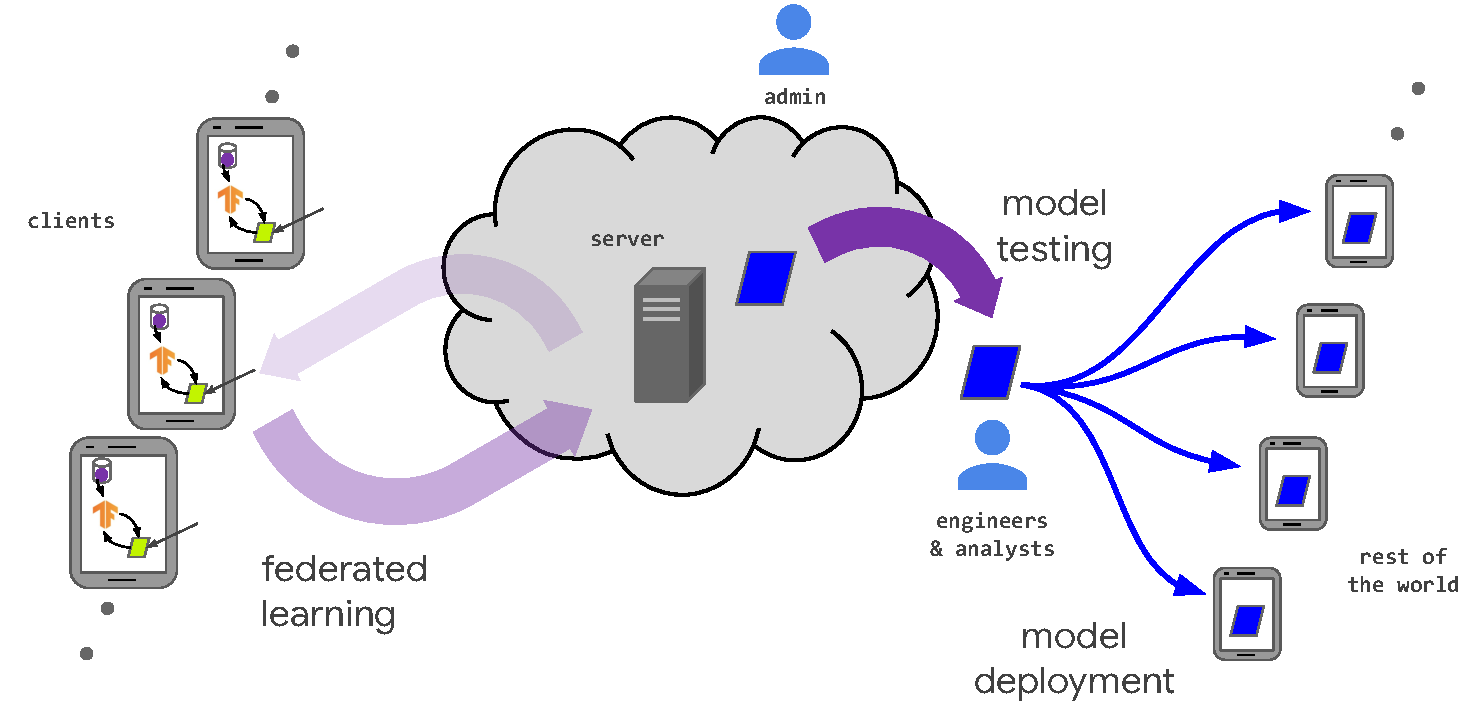
\includegraphics[width=\textwidth]{actors.pdf}
}}

\begin{figure}[ht] 
% Uses the figure saved above.
\noindent\usebox{\actorsfigure}
\caption{The lifecycle of an FL-trained model and the various actors in a federated learning system. This figure is revisited in \cref{sec:privacy} from a threat models perspective. %In the cross-silo FL setting, the clients are organizations (e.g. hospitals or banks) rather than mobile devices.
} 
\label{fig:actors}
\end{figure}

\subsubsection{The Lifecycle of a Model in Federated Learning}\label{sec:lifecycle}
The FL process is typically driven by a model engineer developing a model for a particular application. For example, a domain expert in natural language processing may develop a next word prediction model for use in a virtual keyboard. \cref{fig:actors} shows the primary components and actors. At a high level, a typical workflow is:

\begin{enumerate}

\item \textbf{Problem identification:} The model engineer identifies a problem to be solved with FL.

\item \textbf{Client instrumentation:} If needed, the clients (e.g. an app running on mobile phones) are instrumented to store locally (with limits on time and quantity) the necessary training data. In many cases, the app already will have stored this data (e.g. a text messaging app must store text messages, a photo management app already stores photos). However, in some cases additional data or metadata might need to be maintained, e.g. user interaction data to provide labels for a supervised learning task.

\item \textbf{Simulation prototyping (optional):} The model engineer may prototype model architectures and test learning hyperparameters in an FL simulation using a proxy dataset.

\item \textbf{Federated model training: } Multiple federated training tasks are started to train different variations of the model, or use different optimization hyperparameters. \label{step:fl-train}

\item \textbf{ (Federated) model evaluation:} After the tasks have trained sufficiently (typically a few days, see below), the models are analyzed and good candidates selected. Analysis may include metrics computed on standard datasets in the datacenter, or federated evaluation wherein the models are pushed to held-out clients for evaluation on local client data.

\item \textbf{Deployment:} Finally, once a good model is selected, it goes through a standard model launch process, including manual quality assurance, live A/B testing (usually by using the new model on some devices and the previous generation model on other devices to compare their in-vivo performance), and a staged rollout (so that poor behavior can be discovered and rolled back before affecting too many users). The specific launch process for a model is set by the owner of the application and is usually independent of how the model is trained. In other words, this step would apply equally to a model trained with federated learning or with a traditional datacenter approach.\label{step:deploy}

\end{enumerate}

One of the primary practical challenges an FL system faces is making the above workflow as straightforward as possible, ideally approaching the ease-of-use achieved by ML systems for centralized training. While much of this paper concerns federated training specifically, there are many other components including federated analytics tasks like model evaluation and debugging. Improving these is the focus of \cref{sec:workflows}. For now, we consider in more detail the training of a single FL model (Step~\ref{step:fl-train} above).



\begin{table}
\centering
\renewcommand{\arraystretch}{1.2}
\begin{tabular}{rl}    
\toprule
Total population size                           & $10^6$--$10^{10}$ devices \\
Devices selected for one round of training      & 50 -- 5000 \\
Total devices that participate in training one model  & $10^5$--$10^7$ \\
Number of rounds for model convergence          & 500 -- 10000 \\
Wall-clock training time                        & 1 -- 10 days \\
\bottomrule
\end{tabular}
\caption{Order-of-magnitude sizes for typical cross-device federated learning applications.}
\label{tab:sizes}
\end{table}

\subsubsection{A Typical Federated Training Process}\label{sec:typical-training}
We now consider a template for FL training that encompasses the Federated Averaging algorithm of \citet{mcmahan17fedavg} and many others; again, variations are possible, but this gives a common starting point. 

% TODO - where does this go

A server (service provider) orchestrates the training process, by repeating the following steps until training is stopped (at the discretion of the model engineer who is monitoring the training process):
\begin{enumerate}

  \item \textbf{Client selection:} The server samples from a set of clients meeting eligibility requirements. For example, mobile phones might only check in to the server if they are plugged in, on an unmetered wi-fi connection, and idle, in order to avoid impacting the user of the device.
  
  \item \textbf{Broadcast:} The selected clients download the current model weights and a training program (e.g. a TensorFlow graph~\cite{tensorflow2015-whitepaper}) from the server.
  
  \item \textbf{Client computation:} Each selected device locally computes an update to the model by executing the training program, which might for example run SGD on the local data (as in Federated Averaging).
  
  \item \textbf{Aggregation:} The server collects an aggregate of the device updates. For efficiency, stragglers might be dropped at this point once a sufficient number of devices have reported results. This stage is also the integration point for many other techniques which will be discussed later, possibly including: secure aggregation for added privacy, lossy compression of aggregates for communication efficiency, and noise addition and update clipping for differential privacy.
  
  \item \textbf{Model update:} The server locally updates the shared model based on the aggregated update computed from the clients that participated in the current round.
\end{enumerate}

Table~\ref{tab:sizes} gives typical order-of-magnitude sizes for the quantities involved in a typical federated learning application on mobile devices.

The separation of the client computation, aggregation, and model update phases is not a strict requirement of federated learning, and it indeed excludes certain classes of algorithms, for example asynchronous SGD where each client's update is immediately applied to the model, before any aggregation with updates from other clients. Such asynchronous approaches may simplify some aspects of system design, and also be beneficial from an optimization perspective (though this point can be debated). However, the approach presented above has a substantial advantage in affording a separation of concerns between different lines of research: advances in compression, differential privacy, and secure multi-party computation can be developed for standard primitives like computing sums or means over decentralized updates, and then composed with arbitrary optimization or analytics algorithms, so long as those algorithms are expressed in terms of aggregation primitives.

It is also worth emphasizing that in two respects, the FL training process should not impact the user experience. First, as outlined above, even though model parameters are typically sent to some devices during the broadcast phase of each round of federated training, these models are an ephemeral part of the training process, and not used to make ``live'' predictions shown to the user.  This is crucial, because training ML models is challenging, and a misconfiguration of hyperparameters can produce a model that makes bad predictions. Instead, user-visible use of the model is deferred to a rollout process as detailed above in Step~\ref{step:deploy} of the model lifecycle. Second, the training itself is intended to be invisible to the user --- as described under client selection, training does not slow the device or drain the battery because it only executes when the device is idle and connected to power. However, the limited availability these constraints introduce leads directly to open research challenges which will be discussed subsequently, such as semi-cyclic data availability and the potential for bias in client selection. 


\subsection{Federated Learning Research}\label{sec:fl-research}
The remainder of this paper surveys many open problems that are motivated by the constraints and challenges of real-world federated learning settings, from training models on medical data from a hospital system to training using hundreds of millions of mobile devices. Needless to say, most researchers working on federated learning problems will likely not be deploying production FL systems, nor have access to fleets of millions of real-world devices. This leads to a key distinction between the practical settings that motivate the work and experiments conducted in simulation which provide evidence of the suitability of a given approach to the motivating problem.

本文的其余部分调查了许多受现实世界联邦学习环境约束和挑战驱动的开放问题, 从医院系统医疗数据的培训模型到使用数亿移动设备的培训. 不用说, 大多数研究联邦学习问题的研究人员很可能不会部署生产FL系统, 也不会访问数以百万计的真实世界设备. 这导致了激励工作的实际设置与模拟中进行的实验之间的关键区别, 模拟中进行的实验为激励问题的给定方法的适用性提供了证据. 

This makes FL research somewhat different than other ML fields from an experimental perspective, leading to additional considerations in conducting FL research. In particular, when highlighting open problems, we have attempted, when possible, to also indicate relevant performance metrics which can be measured in simulation, the characteristics of datasets which will make them more representative of real-world performance, etc. The need for simulation also has ramifications for the presentation of FL research. While not intended to be authoritative or absolute, we make the following modest suggestions for presenting FL research that addresses the open problems we describe:


这使得FL研究从实验的角度与其他ML领域有所不同, 导致在进行FL研究时需要额外考虑. 特别是, 在强调开放性问题时, 我们已尝试在可能的情况下, 也指出可在模拟中测量的相关性能指标、数据集的特征, 这些特征将使其更能代表真实世界的性能, 对模拟的需求也对外语研究的呈现产生了影响. 虽然不是为了权威性或绝对性, 但我们提出以下温和的建议, 以展示解决我们描述的开放性问题的外语研究:


\begin{itemize}
    \item As shown in \cref{tab:characteristics}, the FL setting can encompass a wide range of problems. Compared to fields where the setting and goals are well-established, it is important to precisely describe the details of the particular FL setting of interest, particularly when the proposed approach makes assumptions that may not be appropriate in all settings (e.g. stateful clients that participate in all rounds).
    
    \item Of course, details of any simulations should be presented in order to make the research reproducible. But it is also important to explain which aspects of the real-world setting the simulation is designed to capture (and which it is not), in order to effectively make the case that success on the simulated problem implies useful progress on the real-world objective. We hope that the guidance in this paper will help with this.
    
    \item Privacy and communication efficiency are always first-order concerns in FL, even if the experiments are simulations running on a single machine using public data.  More so than with other types of ML, for any proposed approach it is important to be unambiguous about \emph{where computation happens} as well as \emph{what is communicated}.
\end{itemize}

Software libraries for federated learning simulation as well as standard datasets can help ease the challenges of conducting effective FL research; \cref{sec:datasets-and-software} summarizes some of the currently available options. Developing standard evaluation metrics and establishing standard benchmark datasets for different federated learning settings (cross-device and cross-silo) remain highly important directions for ongoing work.

\subsection{Organization}
\cref{sec:relaxing} builds on the ideas in \cref{tab:characteristics}, exploring other FL settings and problems beyond the original focus on cross-device settings. \cref{sec:better_fl} then turns to core questions around improving the efficiency and effectiveness of federated learning.
%
\cref{sec:privacy} undertakes a careful consideration of threat models and considers a range of technologies toward the goal of achieving rigorous privacy protections. As with all machine learning systems, in federated learning applications there may be incentives to manipulate the models being trained, and failures of various kinds are inevitable; these challenges are discussed in \cref{sec:robust}. Finally, we address the important challenges of providing fair and unbiased models in \cref{sec:fairness}.

\cref{sec:privacy}对威胁模型进行了仔细的考虑, 并考虑了一系列旨在实现严格隐私保护目标的技术. 与所有机器学习系统一样, 在联邦学习应用程序中, 可能存在操纵正在训练的模型的动机, 各种各样的失败是不可避免的;这些挑战将在\cref{sec:robust}中讨论. 最后, 我们讨论了在\cref{sec:fairness}中提供公平无偏模型的重要挑战. 

%%%%%%%%%%%%%%%%%%%%%%%%%%%%%%%%%%%%%%%%%%%%%%%%%%%%%%%%%%%%%%%%%%%%%%%%%%%%%%%%%%%%%%
\pagebreak